\section{Social Routing Service}

The Social Routing Service is comprised of three major components, each with it's own purpose. 
A database to store user related information, a server to process data and an API to expose it's functionality.
This logic is represented in FIGURE XXXX TODO.

\begin{figure}[h]            
    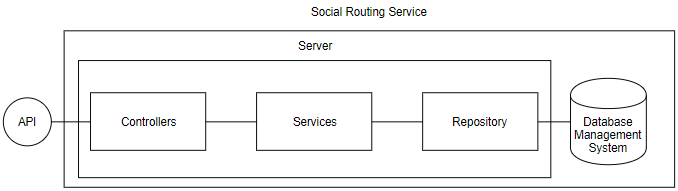
\includegraphics[width=\textwidth]{images/project-structure/service-structure.PNG}
    \caption{Social Routing Service architecture.}
\end{figure}  

\subsection*{Social Routing API}

    \subsection*{Schema}
        The Social Routing API uses the HTTP protocol as a medium to communicate and all the data sent or received 
        must be in the JSON format.

        The base endpoint of the API is : how to present url links?
        !!!WHY HTTP AND WHY JSON?

        Data obtained from the API is either a single resource or a collection of resources. For example, a request
        made to retrieve a route will have as a response a single resource which will contain the representation of that
        route. If a request is made to obtain routes by location then the response will be a collection of resources containing
        the several route representations.
        This single and collection terms when associated with a resource were decisive in the choice of how much data would 
        be returned in either of them. A request for a collection doesn't require detailed information about each element of the
        collection, it needs to provide general information and a form for the API user to retrieve detailed information about a specific 
        collection element. 
        With this idea in mind the resource representations were divided into two types, a detailed representation for when a user
        requests a single resource and summary representation for each element inside a requested collection, containing only the 
        information about that element that is necessary.

        Example of a detailed resource, when requesting a single route:

        \begin{lstlisting}
{
"identifier": 1,
"location": "location 1",
"name": "name 1",
"description": "description 1",
"rating": 5,
"duration": 1,
"dateCreated": "2019-05-26",
"points": [
    {
        "latitude": 3,
        "longitude": 4
    },
    {
        "latitude": 3,
        "longitude": 4
    }
],
"categories": [
    {
        "name": "Sea"
    }
],
"ownerUrl": "http://host/api.sr/persons/1"
}
        \end{lstlisting}

        Example of a collection of resources, being that each collection element is in it's summary resource representation, when
        requesting the routes of a user:
        
        \begin{lstlisting}
{
"routes": [
    {
        "identifier": 1,
        "name": "name 1",
        "rating": 5,
        "routeUrl": "http://host/api.sr/routes/1"
    }
]
}
        \end{lstlisting}
    
    \newpage
    
    \subsection*{Authentication}
    The API's authentication is made with the support of the Google Sign-In API. The authentication with the API is done in two phases.
    The first phase is the registration of a new user. On this phase a POST request must be made to the endpoint:\\ 
    \textit{http://api.sr/sign-in/google?idTokenString=googleIdTokenString}.\par
    Where the googleIdTokenString is the token provided by the Google Sign-In API. When the token is received in the Service's API, it's authenticity is verified using the Google Sign-in-API. 
    After the validity of the token is verified the subject field is extracted from it to identify the user performing the registration and stored by the service. 
    Then an API token is generated from a time based uuid generator, provided by the Log4J library, and associated to the previously received subject. 
    Before being stored the token is hashed to increase security. The response to the request will contain both the generated token (in it's original form) 
    and subject, so the user haves the required information to make authenticated requests from there on.\par

    The second phase of the authentication process is made in any request that follows user registration. The API user must send a request containing the previously 
    received token and subject in the Authorization and Subject HTTP headers respectively.\par
    When any request is received the headers are retrieved, and checked against the service's database. In this check, the received token is hashed and 
    compared to the hashed version on the database associated to that subject. If either of them is not present or not associated
    with each other then the authentication fails and the user receives an error response.

    \subsection*{Supported HTTP Methods}
        Due to the nature of the HTTP protocol, the API supports four different HTTP request methods: GET, POST, PUT and DELETE. This chapter describes each method and provides
        examples for each of them.
        
        \subsubsection*{GET}
            This method is used to retrieve resources from the API. The following request retrieves a resource representing
            a person resource with the identifier 1.\par
            
            GET http://api.sr/persons/1

            The response to this request would be:\newline
        \begin{lstlisting}
{
"identifier": 1,
"rating": 4,
"routesUrl": "http://api.sr/persons/1/routes"
}
        \end{lstlisting}

        \subsubsection*{POST}
            The POST HTTP method is used to create resources. It requires that the Content-Type HTTP header is defined and with the value 
            \textit{application/json}. The following request creates a route owned by the person with identifier 1.\par
            
            POST http://api.sr/routes
            
            And in the body of the request, the route to be created must be described:\newline
            \begin{lstlisting}
{
"location": "location 1",
"name": "name 1",
"description": "description 1",
"points": [
    {
        "latitude":3,
        "longitude":4
    },
    {
        "latitude":3,
        "longitude":4
    }
],
"categories" : [
    {
        "name" : "Sports"
    }
],
"personIdentifier": 1
}
            \end{lstlisting}
            
            The response to this request will have an empty body and return the location of the created resource in the Location header of the response. If successful
            the status code of the response is 201.  

        \subsubsection*{PUT}
        The PUT method is used to replace or update a resource or a collection of resources. Like the post request it requires that the
        request contains the HTTP header Content-Type defined with \textit{application/json}.
        The following request replaces the currently existing resource route with identifier 1 with the one sent in the body of the request.

        PUT http://api.sr/routes/1

        Request body:
        \begin{lstlisting}                
{
"location": "location 1",
"name": "name 1",
"description": "description 1",
"rating": 1.0,
"duration": 1000,
"points":[
    {
    "latitude": 3.0,
    "longitude": 1.0
    }
],
"categories":[
    {
        "name":"Sports"
    },
    {
        "name":"Sea"
    }
]
}
        \end{lstlisting}
        A successful response will have the 200 OK status and an empty body.

        \subsubsection*{DELETE}
        DELETE, as the name implies is utilized to delete a resource. The following request deletes a route with 1 as identifier.\\
        DELETE http://api.sr/routes/1

        A successful response will have the 200 OK status and an empty body.
    
    \subsection*{Pagination}
    Requests that return a collection of resources will be paginated to a default value of 5 resources within the collection. 
    A specific page can be requested with the query parameter \textit{?page={number}}. 
    The following request returns the first five routes that a person with identifier 1 created:\\
    GET http://api.sr/persons/1/routes?page=1\\
    To obtain the next 5 one would simply change de value of page to 2.

    \subsection*{Errors}
    The error responses follow the RFC standard of type problem+json. The structure of an error response is the following:
    \begin{lstlisting}
{
"type": "(string) A URI reference that identifies the problem type.",
"title": "(string)A short summary of the problem type.",
"status": "(number) The HTTP status code for this problem.",
"detail": "(string) An explanation specific to this occurrence of the problem. (Optional)",
"instance" : "(string) A URI reference that identifies the specific occurrence of the problem. (Optional)",
}
    \end{lstlisting}

    \subsubsection*{Hypermedia}
    Some resources have links to other resources. Either to a parent resource or to a detailed representation of a 
    resource within a collection. For example, a user resource might have a link to their created routes, which 
    holds a collection of routes. That same collection might have a link to the profile of the person who created 
    the routes.

\subsection*{Server} 
The server uses Kotlin as a programming language and the Spring framework to expose a REST service.
It's role within the system is data receival, data processing, and to respond acordingly.
It is divided in three major layers, each with it's role in the Social Routing Service's system. 
They are the Controllers, the Services and the Repository.\\

The Controllers are responsible for handling the reception of an HTTP request to the service and are mapped to
it's endpoints. Upon receiving a request they will use the available services to perform desired operations either
over a set of received data or to generate the requested data.\\

The Services are responsible for processing data and communicating the the Repository layer.\\

The Repository layer is the only layer with direct access to the database and as such is responsible for communicating
with it. The communication is made through the use of JDBI, a library built on top of the driver JDBC. This allows
less verbose code while maintaining control over SQL queries.\\ 

Besides these three major layers the server contains other important components, the Interceptor and the Exception Handler.
There are three different implementations of the Interceptor component.\\

The Authentication Interceptor is responsible for user authentication before the request reaches a controller. The goal of this
implementation is to avoid server overhead, resolving the authentication before the request is processed allows for a fast response
if the user is incorrectly authenticated instead of continuing with the unnecessary processing of data.\\

The Logging Interceptor is used both before and after the request is processed to provide information regarding each request for debugging
purposes.\\

The Media Type Interceptor is used, like the Authentication Interceptor, to avoid overhead, since if a post request is made
with wrong Content-Type headers or no headers at all then the service does not support that request and can respond with an 
error immediately.\\

The Exception Handler is the component responsible for the handling of exceptions of the system. In the Spring framework there 
are several ways to handle exceptions, but the choice to make is to either handle the exceptions locally or globally. The 
handler implementation groups all the exceptions thrown by the system in a single class and produces their respective error 
messages. It allows for an easier work flow when treating exceptions. The global handling was chosen because most of the 
exceptions happen in more than one endpoint and would produce a lot of repeated code if handled locally.\\      

As an example, the flow of a correct HTTP POST request to the routes resource that arrives on the server is the following:
    \begin{itemize}
        \item The request is intercepted by the Logging Interceptor and logs the request information.
        \item It is then intercepted by the Media Type Interceptor, that checks if the request data format received is supported by the service.
        \item The Authentication Interceptor checks the user credentials to see if the user can indeed access the service.
        \item The endpoint is reached in it's mapped Controller, which receives the Route information and that it maps to the correct object. In this case the Route Controller which will then call a service responsible for processing the request data.
        \item The service, in this case Route Service, will process the data and map it  to the correct data type and make a request to the repository to store the received data.
        \item The repository communicates with the database, to which it sends the data in a database accepted format.
        \item The database stores the data and returns the identifier of the newly created Route.
        \item The repository receives the identifier and passes it through to the Route Service.
        \item The Service passes the received information to the Route Controller.
        \item The Route Controller builds the newly created route resource URI with the received Route identifier and maps it to the header Location of the response and returns.
    \end{itemize}

\subsection*{Database Management System}
The database management system chosen was PostgreSQL, using the hybrid functionality of storing valid JSON directly in a table
 field. The database is used to store all entities required for the service to function and to deliver them to repositories in need. 
The decision of choosing JSON as a type to store data comes with the need of storing large sets of coordinates belonging to a single entity, 
this will allow us to make faster and easier calculations of times and distances between routes and points rather than if a Point was it's own database entity. 

The database entity diagram is shown in figure TODO FIGURE reference.

\begin{figure}[h]            
    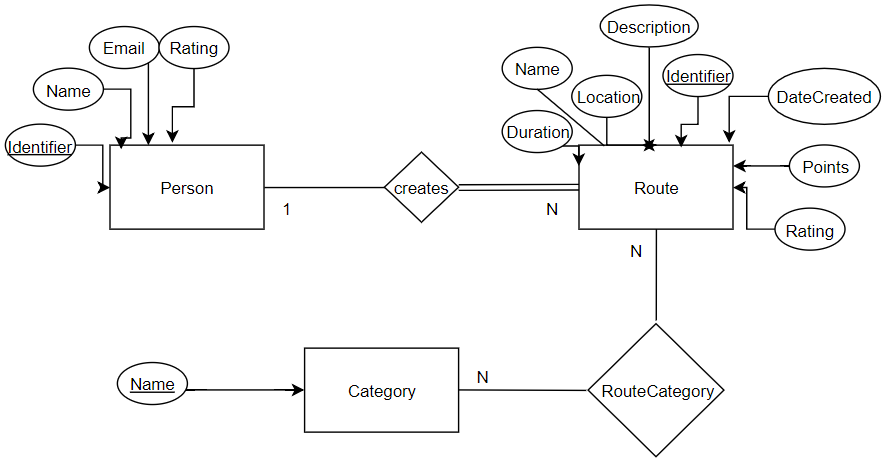
\includegraphics[width=\textwidth]{images/project-structure/dbms-structure.PNG}
    \caption{Entity Relationship Diagram.}
\end{figure}   
